%************************************************
\chapter{Implementation}\label{ch:implementation}
%************************************************

\begin{itemize}

\item{
	Intro text describing what is implemented, features, hardware
}
\item{
	Show user interface and describe mechanics. how to speech and gesture. mention activation angle study and show plot. 
}
\item{
	Mention Modules and communicationManager. show communication protocol. maybe uml diagram of whole application
}
\item{
	Describe Handheld module. introduce spotify api + webapi wrapper.
}
\item{
	Describe Wear module
}
\item{
	possible improvements and restrictions to the program (like leaving out unneeded spotify features), input feedback
}

\end{itemize}

This chapter describes the smartwatch controlled mobile music player implementation. It gives an insight into the chosen interaction techniques, the mobile-wear communication and the core music player functions.

The essential music library is provided by a private Spotify\footnote{Music streaming service: \url{www.spotify.com}} premium account. The prototype is divided into two separate applications, i.e. mobile (handheld) and wear (smartwatch). Users are able to access all features of the mobile application via the smartwatch application. In order to make use of the focused-casual continuum \cite{pohl2013focused}, three interaction techniques, differing in the amount of control granted, are available for the user:
\begin{itemize}
\item{Touch}
\item{Speech}
\item{Gesture}
\end{itemize}
Each technique can be used for the simpler actions of the music player such as play and pause, skip to previous or next song and changing the volume. However, for the more complex interactions, e.g. choosing a playlist, only the touch and speech interaction methods suffice. Gesture and speech input can be performed casually while not even looking at the device (the smartwatch). The following section describes the functionality and the power of the different methods.

Both applications are implemented for the android platform. The handheld device has no further hardware or software requirements other than supporting the android wearable \ac{API} so a Samsung Galaxy S6 is chosen. The smartwatch application certainly requires the device to be equipped with a acceleration sensor and a microphone. A moto360 from Motorola is well suited for this. Both devices need to support Bluetooth, too.

\section{User Interface}
The \ac{GUI} from the mobile application only differs from the wear \ac{GUI} in terms of appearance. In terms of control over the music player, both versions offer the same possibilities and show the same information (when connected) at any given time. The wear application, however, additionally introduces speech and gesture interactions which the mobile application is not capable of.

It is noteworthy that the Spotify \ac{SDK} offers a lot more functionality than implemented, such as creating own playlists or searching the entire Spotify music library for keywords. The implemented music player, however, just offers the basic playback functionalities in order to keep the application simple and to not overload the experiment participants with information since they have to remember how to control the music player.

\subsection{Touch Input - \ac{GUI}}
Both \ac{GUI}s are designed to be simple and straightforward. The mobile version mainly consists of two areas. Figure \ref{fig:mobileGUI} depicts a screenshot of this layout. A control panel is situated at the bottom of the screen. Above this is a left-right scrollable pager containing different kinds of lists. \marginpar{Categories are Spotify's extended version of genres} The scrollable list pager contains five lists, one for each music arrangement which are playlists, songs, albums, artists and categories.
\begin{figure}[bth]
	\myfloatalign
	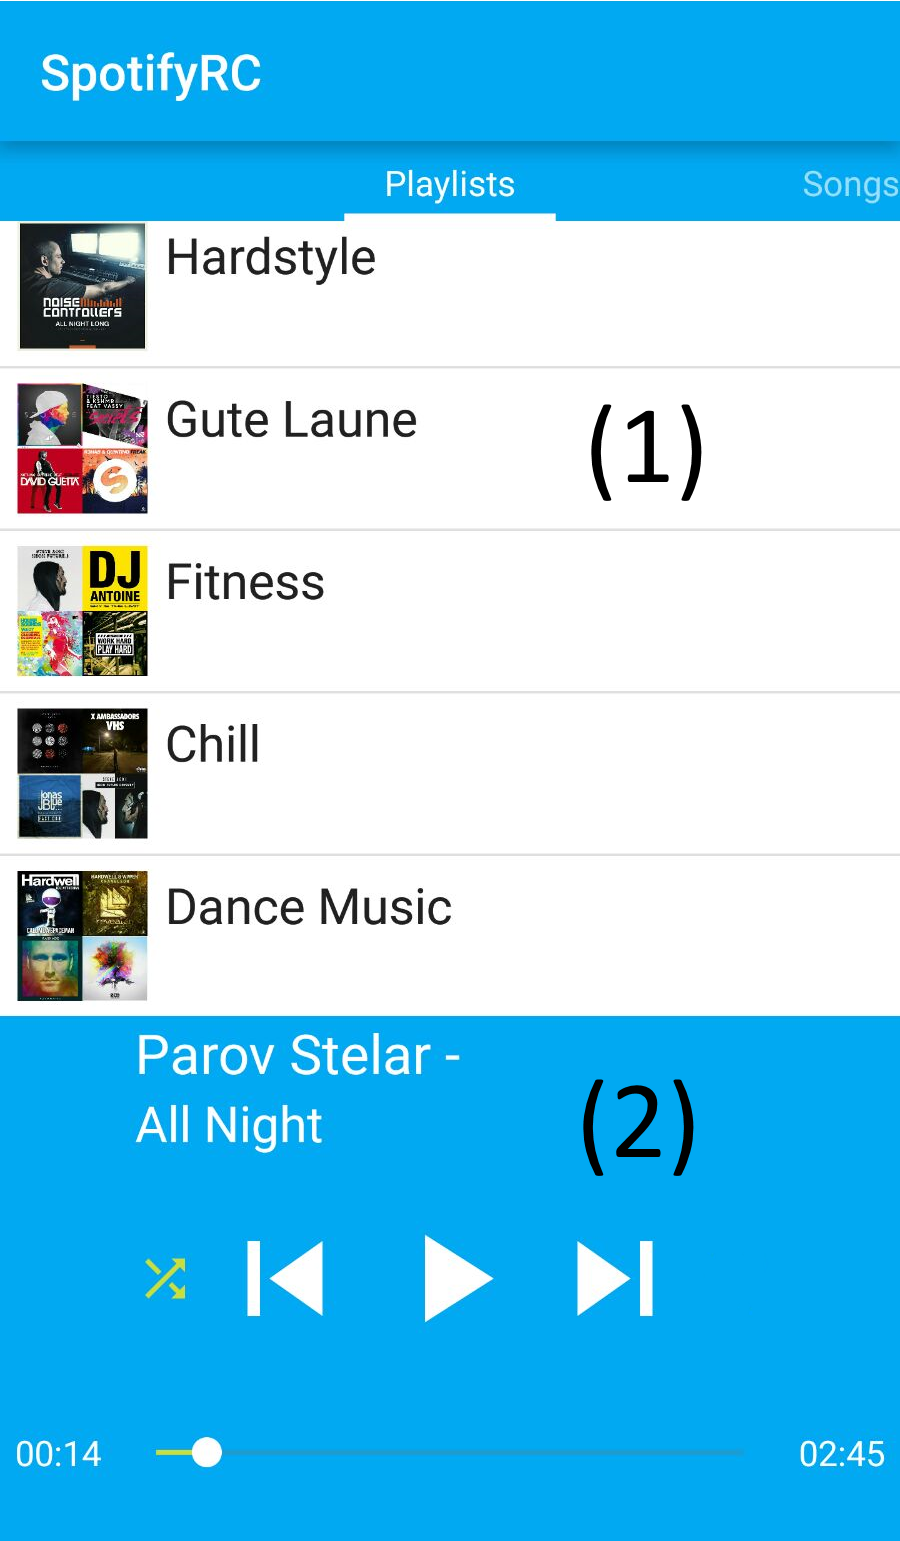
\includegraphics[width=.45\linewidth]{img/mobileGUIlabeled.png}
	\caption{\ac{GUI} of the mobile application. (1) shows the left-right scrollable list pager with indicators which list is shown at the top. (2) shows the player control panel in blue.}
	\label{fig:mobileGUI}
\end{figure}
The control panel located beneath the list pager contains four control buttons such as a shuffle button including on-off indicator, a skip to previous song button, a play-pause button and a skip to next song button. Unlike the wear application, the mobile version spares buttons for controlling the volume, because most devices own hardware buttons for this purpose. Information on the name of the current song and artist can be found above these buttons. The track's progress and total duration can be found at the very bottom of the screen. \\

However, the intention of the wear application is, that the user does not need to bother reaching his mobile phone. For this reason, the wear application's \ac{GUI} offers the same amount of touch control over the music player. Figure \ref{fig:wearGUI} demonstrates the layout of the wear application. It consists of a GridViewPager with three horizontal pages. 

\begin{figure}[bth]
	\myfloatalign
	\subfloat[control panel in interactive mode]
	{\label{fig:wearGUI-controls}
	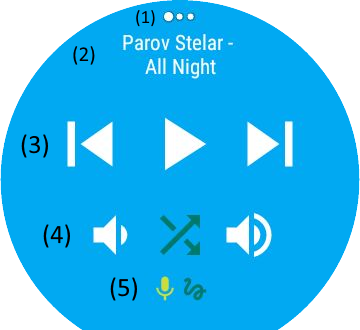
\includegraphics[width=.3\linewidth]{img/wearGUIcontrolsPage.png}} \quad
	\subfloat[list of music arrangements]
	{\label{fig:wearGUI-select}
	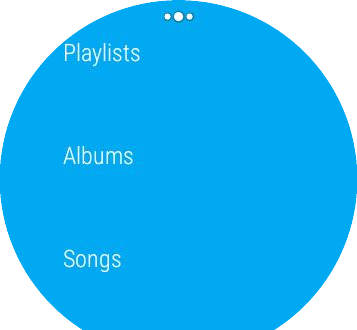
\includegraphics[width=.3\linewidth]{img/wearGUIselect.png}} \quad
	\subfloat[list of playlists]
	{\label{fig:wearGUI-items}
	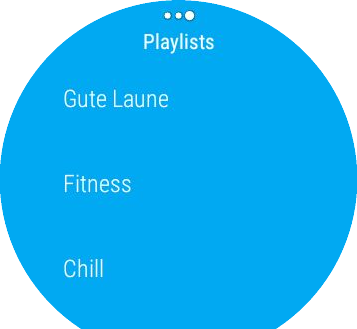
\includegraphics[width=.3\linewidth]{img/wearGUIitems.png}} \\
	\subfloat[control panel in ambient mode]
	{\label{fig:wearGUI-ambient}
	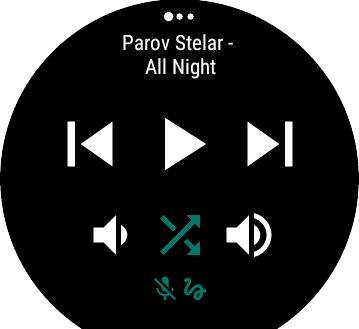
\includegraphics[width=.3\linewidth]{img/wearGUIambient.png}}
	\caption{ The \ac{GUI} of the wear application consists of a GridViewPager containing three horizontal pages. A dot indicator at the top of the screen shows the current page. \ref{fig:wearGUI-ambient} depicts the controls page in ambient mode, i.e. battery saving mode, while \ref{fig:wearGUI-controls} is the same screen in interactive mode. Swiping right brings up the list of music arrangements \ref{fig:wearGUI-select}. Selecting e.g. playlists switches to the third page \ref{fig:wearGUI-items} showing a list with all playlists.}
	\label{fig:wearGUI}
\end{figure}

Figure \ref{fig:wearGUI-controls} shows the main control page which is divided into five rows (1) - (5). A dot indicator showing the current page with a bigger dot is located at the top of the screen in row (1). Row (2) contains the current artist and track that is playing. Row (3) and (4) contain the control buttons, i.e. in (3) the buttons for play previous song, toggle play and pause, play next song and in (4) the buttons for decrease volume, toggle shuffle (grey = off, green = on) and increase volume are located. Row (5) contains two icons which indicate whether speech and gesture recognition are active (green) or inactive (grey).

Figure \ref{fig:wearGUI-select} shows the page in the middle which is reached by swiping over the screen from right to left. The page contains a vertical scrollable list of the five music arrangements, namely playlists, songs, albums, artists and categories. Selecting a list entry scrolls to the right (the third) page which always adapts its list showing the respective items in the selected arrangement. \\

The moto360 smartwatch is equipped with a battery saving mode called ambient mode. In this mode cpu processing is reduced and it is recommended\footnote{\url{https://developer.android.com/training/wearables/apps/always-on.html}} to reduce the \ac{UI} layout to a black background and white text color. Updates to the \ac{UI} should then happen on a several seconds up to a minute basis. Applications that run in both ambient and interactive mode are called \textit{always-on apps}. The transition from interactive to ambient mode happens either automatically after a short period of user inactivity or can be forced by covering the screen. Leaving ambient mode happens either by touching the screen or by bringing up the wrist as in looking at the time. Figure \ref{fig:wearGUI-ambient} depicts the control page of the wear application running in ambient mode with a black background and white text and icon color. \\

\subsection{Speech Control}
The wear application offers the possibility to control the music player via speech commands. In order to enter a speech command, the application must be in interactive mode which activates the continuous speech recognition (indicated by the green microphone in \ref{fig:wearGUI-controls} at the bottom of the screen). The user can then talk to the watch and issue a command. Speech data is recorded and converted to text by the android speech recognition service\footnote{\url{https://developer.android.com/reference/android/speech/SpeechRecognizer.html}}.  The converted text is then send to the mobile application where it is parsed, transformed into a command and finally executed.
\begin{figure}[bth]
	\myfloatalign
	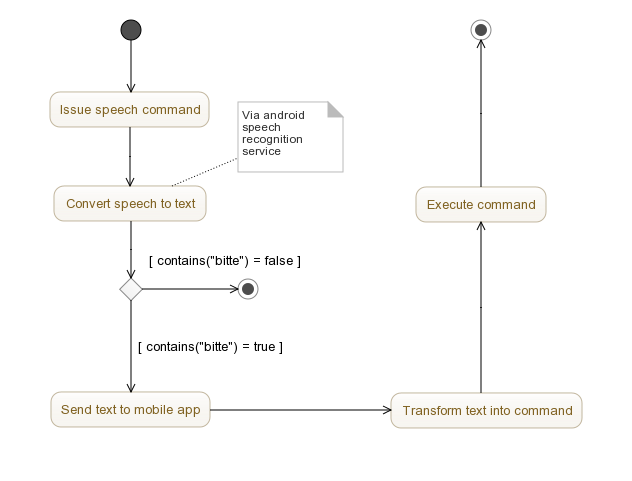
\includegraphics[width=.99\linewidth]{img/SpeechActivityDiagram.png}
	\caption{Lorem Ipsum}
	\label{fig:speechAD}
\end{figure}

\subsection{Gesture Control}

%Chapter \ref{ch:implementation} 


%*****************************************
%*****************************************
%*****************************************
%*****************************************
%*****************************************




